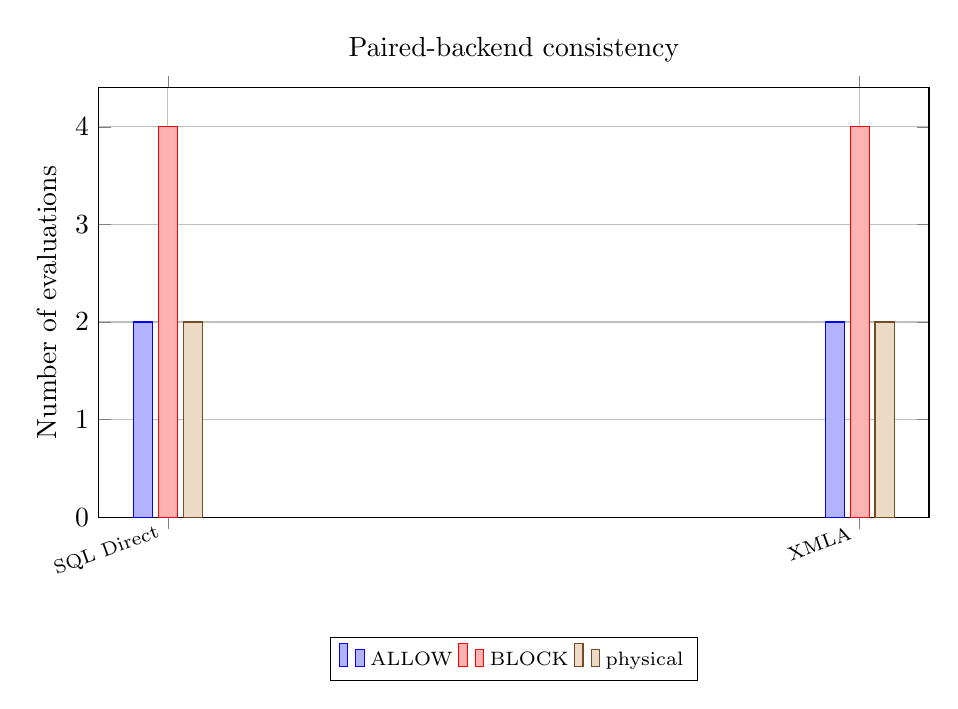
\begin{tikzpicture}
\begin{axis}[ybar,
bar width=7pt,
width=\linewidth,
height=0.58\linewidth,
title={Paired-backend consistency},
ylabel={Number of evaluations},
xtick={0,1},
xticklabels={{SQL Direct},{XMLA}},
x tick label style={rotate=20,anchor=east,font=\scriptsize},
grid=major,
legend style={font=\scriptsize,at={(0.5,-0.28)},anchor=north,legend columns=3},
ymin=0]
\addplot+ coordinates {(0,2) (1,2)};
\addlegendentry{ALLOW}
\addplot+ coordinates {(0,4) (1,4)};
\addlegendentry{BLOCK}
\addplot+ coordinates {(0,2) (1,2)};
\addlegendentry{physical}
\end{axis}
\end{tikzpicture}
